\section{Introduction to the Patterns}

Die vier Phasen des Lebenszyklus eines Fehlers sind:
\begin{itemize}
	\item error detection
	\item error recovery
	\item error mitigation
	\item fault treatment
\end{itemize}

Diese spielen wie folgt zusammen:

\begin{figure}[H]
	\centering
	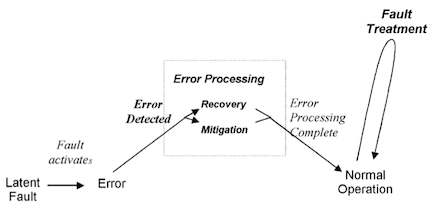
\includegraphics[width=\textwidth]{content/faulttolerance/images/introduction_four_phases_of_fault_tolerance.png}
	\caption{introduction four phases of fault tolerance}
\end{figure}


\subsection{Shared Context for These Patterns}

Die Patterns zielen auf folgende Attribute ab

\subsubsection*{Real-Time}

Zwei unterschiedliche Varianten
\begin{itemize}
	\item soft real-time: Beispiel Webserver antwortet direkt auf Anfrage, ist jedoch nicht schlimm wenn es mal länger dauert
	\item hard real-time: Beispiel Flugzeug, falls ein Kontrollsystem nicht in Echtzeit reagiert kann dies katastrophale Folgen haben
\end{itemize}

\subsubsection*{State or Stateless}

\begin{itemize}
	\item stateless, eine Anfrage wird verarbeitet und ist danach nicht mehr Teil des Systems
	\item stateful, Systeme dessen Verarbeitung längere Zeit in Anspruch nehmen und sich Daten merken müssen
\end{itemize}

\subsubsection*{External Observers}

Oft besitzen Fehlertolerante Systeme Observer bzw. Monitoring Teile welche Informationen über aufgetretene Fehler sammeln. Dies ist eine wichtige Anforderung an das System, da dadurch Fehler analysiert und reduziert werden können.

\subsubsection*{Integrated Fault Tolerance}

Meist ist die Fehlerbehandlung in Programm integriert, dies macht es schwierig eine Fehlerbehandlung in anderen Situationen wieder zu verwenden.

\subsubsection*{Fault Tolerance is Not Free}

Behalte im Hinterkopf das eine Fehlerbehandlung meist nicht gratis ist, z.B. braucht eine redundante Daten Kopie zusätzlichen Speicher.

\subsubsection*{Long Lived Systems}

Lang lebend = höhere Entwicklungskosten = Erwartung das Fehler Tolerant

\subsection{Terminology}

Ein "System" besteht aus "Komponenten" ("Klassen" oder "Module"), diese Komponenten laufen in oder enthalten verschiedene "Tasks", diese wiederum laufen auf eine Einheit von Hard- oder Software. Solange keine Fehler den Verlauf eines Systems stören, nennt man dies "normal processing". Wenn ein System mit unterschiedlichen Komponenten zusammenarbeitet nennt man diese "peers".



\subsection{Fragen}

\begin{enumerate}
	\item Wie heissen die vier Phasen eines Faults?
	\begin{itemize}
		\item error detection
		\item error recovery
		\item error mitigation
		\item fault treatment
	\end{itemize}

	\item Weshalb ist Fault Tolerance nicht gratis?
	\begin{itemize}
		\item Redundanz kostet Speicher
		\item Monitoring kostet Rechenleistung
	\end{itemize}

\end{enumerate}

